\documentclass[12pt,
brazilian,
a5paper]{abntex2} % Default font size and left-justified equations

%%%%%%%%%%%%%%%%%%%%%%%%%%%%%%%%%%%%%%%%%
% The Legrand Orange Book
% Structural Definitions File
% Version 2.1 (26/09/2018)
%
% Original author:
% Mathias Legrand (legrand.mathias@gmail.com) with modifications by:
% Vel (vel@latextemplates.com)
%
% This file was downloaded from:
% http://www.LaTeXTemplates.com
%
% License:
% CC BY-NC-SA 3.0 (http://creativecommons.org/licenses/by-nc-sa/3.0/)
%
%%%%%%%%%%%%%%%%%%%%%%%%%%%%%%%%%%%%%%%%%

% % ----------------------------------------------------------------------------------------
% %	VARIOUS REQUIRED PACKAGES AND CONFIGURATIONS
% % ----------------------------------------------------------------------------------------

% \hypersetup{pdftitle={Title},pdfauthor={Author}} % Uncomment and fill out to include PDF metadata for the author and title of the book

% \usepackage{mathtools}
% \usepackage{amsfonts}
% \usepackage{mathrsfs} % para mathscr

\usepackage{ifxetex}
\ifxetex
% % se for utilizar as fontes do sistema: **escolha sua fonte**
% comandos de fontes
\usepackage{mathspec}
\setmathsfont(Digits,Latin,Greek){Minion Pro}
\setmathrm{Minion Pro}
\setmainfont[Numbers=OldStyle]{Minion Pro} %fonte principal (serifada)
\setsansfont[Scale=0.9]{Myriad Pro} %fonte sem serifas
\setmonofont[Scale=MatchLowercase]{Consolas} % fonte monoespaçada

\usepackage{polyglossia} %always load polyblossia after fonts for digits in math mode
\setmainlanguage{brazil}
\setotherlanguages{french,english,spanish,german,italian}

\else
% % se for utilizar pdflatex
% \usepackage[utf8]{inputenc}
% \usepackage{newtxmath}
% \usepackage{Alegreya}
% \usepackage{AlegreyaSans}
\usepackage[nf]{coelacanth}
\usepackage[T1]{fontenc}
%% The font package uses mweights.sty which has som issues with the
%% \normalfont command. The following two lines fixes this issue.
\let\oldnormalfont\normalfont
\def\normalfont{\oldnormalfont\mdseries}
\usepackage[lf]{FiraMono}
\usepackage[italic]{mathastext}
\usepackage{slantsc}
\fi


%% Observação: o pacote polyglossia pode apresentar erro ao ser utilizado com ifxetex + babel.
%% Se isso acontecer, atualize o pacote para a versão mais recente ou utilize somente uma das sequências (pdflatex ou xelatex), comentando ou apagando a outra.

\usepackage{microtype} 				% para melhorias de justificação
% \usepackage[dvipsnames]{xcolor} 		% para cores
% \usepackage{graphicx} 			% para imagens
\usepackage{booktabs,tabularx,rotating}	% para tabelas
\usepackage{mdframed} 				% para caixas de texto como na CIP do verso do título
\usepackage{multicol}				% tabelas com colunas mescladas
\usepackage{lettrine}				% letras capitulares
\usepackage{xspace} 				% para nao precisar de espaços com {} depois de comandos
% como \LaTeX e abreviações criadas pelo usuário
\usepackage{lipsum} 				% para texto de preenchimento de exemplo
\usepackage{leading}				% espaçamento entrelinhas (leading)
\leading{13pt}

% ---
% Pacotes de citações
% ---
\usepackage[brazilian,hyperpageref]{backref}	 % Paginas com as citações na bibl
\usepackage[alf]{abntex2cite}	% Citações padrão ABNT

% ---
% Configurações do pacote backref
% Usado sem a opção hyperpageref de backref
\renewcommand{\backrefpagesname}{Citado na(s) página(s):~}
% Texto padrão antes do número das páginas
\renewcommand{\backref}{}
% Define os textos da citação
\renewcommand*{\backrefalt}[4]{
  \ifcase #1 %
  Nenhuma citação no texto.%
  \or
  Citado na página #2.%
  \else
  Citado #1 vezes nas páginas #2.%
  \fi}%
% ---


%% Spacing of general text; among lines, chapter, section etc
\setlength{\parindent}{1.3em}
\setlength{\parskip}{0.2em}
\renewcommand{\baselinestretch}{1.0}


\usepackage{graphicx} % Required for including pictures
\graphicspath{{Pictures/}} % Specifies the directory where pictures are stored

\usepackage{lipsum} % Inserts dummy text

\usepackage[edges]{forest}    %%Hierarchy Diagram
\usetikzlibrary{shadows.blur}

\usepackage{tikz} % Required for drawing custom shapes

% \usepackage[brazilian]{babel} % English language/hyphenation

\usepackage{enumitem} % Customize lists
\setlist{nolistsep} % Reduce spacing between bullet points and numbered lists

\usepackage{booktabs} % Required for nicer horizontal rules in tables

\usepackage{xcolor} % Required for specifying colors by name
\definecolor{ocre}{RGB}{243,102,25} % Define the orange color used for highlighting throughout the book

% % \usepackage{abntex2}

% % ----------------------------------------------------------------------------------------
% %	MARGINS
% % ----------------------------------------------------------------------------------------

\usepackage{geometry} % Required for adjusting page dimensions and margins

\geometry{
  paper=a4paper, % Paper size, change to letterpaper for US letter size
  top=2cm, % Top margin
  bottom=2cm, % Bottom margin
  left=2.3cm, % Left margin
  right=2.3cm, % Right margin
  headheight=3pt, % Header height
  footskip=1.5cm, % Space from the bottom margin to the baseline of the footer
  headsep=1cm, % Space from the top margin to the baseline of the header
  % showframe, % Uncomment to show how the type block is set on the page
}

% % ----------------------------------------------------------------------------------------
% %	FONTS
% % ----------------------------------------------------------------------------------------

% \usepackage{lmodern}	% Usa a fonte Latin Modern
% \usepackage{avant} % Use the Avantgarde font for headings
% % \usepackage{times} % Use the Times font for headings
% \usepackage{mathptmx} % Use the Adobe Times Roman as the default text font together with math symbols from the Sym­bol, Chancery and Com­puter Modern fonts

% \usepackage{microtype} % Slightly tweak font spacing for aesthetics
% \usepackage[utf8]{inputenc} % Required for including letters with accents
% \usepackage[T1]{fontenc} % Use 8-bit encoding that has 256 glyphs
\usepackage{indentfirst}		% Indenta o primeiro parágrafo de cada seção.

% % ----------------------------------------------------------------------------------------
% %	BIBLIOGRAPHY AND INDEX
% % ----------------------------------------------------------------------------------------

% \usepackage[style=numeric,citestyle=numeric,sorting=nyt,sortcites=true,autopunct=true,babel=hyphen,hyperref=true,abbreviate=false,backref=true,backend=biber]{biblatex}
% \addbibresource{bibliography} % BibTeX bibliography file
% \defbibheading{bibempty}{}

% ---
% Pacotes de citações
% ---
\usepackage[brazilian,hyperpageref]{backref}	 % Paginas com as citações na bibl
\usepackage[alf]{abntex2cite}	% Citações padrão ABNT
\usepackage{abntex2abrev}
% ---
% CONFIGURAÇÕES DE PACOTES
% ---

% ---
% Configurações do pacote backref
% Usado sem a opção hyperpageref de backref
\renewcommand{\backrefpagesname}{Citado na(s) página(s):~}
% Texto padrão antes do número das páginas
\renewcommand{\backref}{}
% Define os textos da citação
\renewcommand*{\backrefalt}[4]{
  \ifcase #1 %
  Nenhuma citação no texto.%
  \or
  Citado na página #2.%
  \else
  Citado #1 vezes nas páginas #2.%
  \fi}%
% ---

\usepackage{calc} % For simpler calculation - used for spacing the index letter headings correctly
\usepackage{makeidx} % Required to make an index
\makeindex % Tells LaTeX to create the files required for indexing

% ----------------------------------------------------------------------------------------
%	MAIN TABLE OF CONTENTS
% ----------------------------------------------------------------------------------------

\usepackage{titletoc} % Required for manipulating the table of contents

\contentsmargin{0cm} % Removes the default margin

% Part text styling (this is mostly taken care of in the PART HEADINGS section of this file)
\titlecontents{part}
[0cm] % Left indentation
{\addvspace{13pt}\bfseries} % Spacing and font options for parts
{}
{}
{}

% Chapter text styling
\titlecontents{chapter}
[1.25cm] % Left indentation
{\addvspace{20pt}\large\sffamily\bfseries} % Spacing and font options for chapters
{\color{ocre!60}\contentslabel[\Large\thecontentslabel]{1.5cm}\color{ocre}} % Formatting of numbered sections of this type
{\color{ocre}} % Formatting of numberless sections of this type
{\color{ocre!60}\normalsize\;\titlerule*[.5pc]{.}\;\thecontentspage}

% Formatting of the filler to the right of the heading and the
% page number

% Section text styling
\titlecontents{section}
[1.25cm] % Left indentation
{\addvspace{1pt}\sffamily\bfseries} % Spacing and font options for sections
{\contentslabel[\thecontentslabel]{1.25cm}} % Formatting of numbered sections of this type
{} % Formatting of numberless sections of this type
{\hfill\color{black}\thecontentspage} % Formatting of the filler to the right of the heading and the page number

% Subsection text styling
\titlecontents{subsection}
[1.25cm] % Left indentation
{\addvspace{1pt}\sffamily\small} % Spacing and font options for subsections
{\contentslabel[\thecontentslabel]{1.25cm}} % Formatting of numbered sections of this type
{} % Formatting of numberless sections of this type
{\ \titlerule*[.5pc]{.}\;\thecontentspage} % Formatting of the filler to the right of the heading and the page number

% Figure text styling
\titlecontents{figure}
[1.25cm] % Left indentation
{\addvspace{1pt}\sffamily\small} % Spacing and font options for figures
{\thecontentslabel\hspace*{1em}} % Formatting of numbered sections of this type
{} % Formatting of numberless sections of this type
{\ \titlerule*[.5pc]{.}\;\thecontentspage} % Formatting of the filler to the right of the heading and the page number

% Table text styling
\titlecontents{table}
[1.25cm] % Left indentation
{\addvspace{1pt}\sffamily\small} % Spacing and font options for tables
{\thecontentslabel\hspace*{1em}} % Formatting of numbered sections of this type
{} % Formatting of numberless sections of this type
{\ \titlerule*[.5pc]{.}\;\thecontentspage} % Formatting of the filler to the right of the heading and the page number

% ----------------------------------------------------------------------------------------
%	MINI TABLE OF CONTENTS IN PART HEADS
% ----------------------------------------------------------------------------------------

% Chapter text styling
\titlecontents{lchapter}
[0em] % Left indentation
{\addvspace{15pt}\large\sffamily\bfseries} % Spacing and font options for chapters
{\color{ocre}\contentslabel[\Large\thecontentslabel]{1.25cm}\color{ocre}} % Chapter number
{}
{\color{ocre}\normalsize\sffamily\bfseries\;\titlerule*[.5pc]{.}\;\thecontentspage} % Page number

% % Section text styling
\titlecontents{lsection}
[0em] % Left indentation
{\sffamily\small} % Spacing and font options for sections
{\contentslabel[\thecontentslabel]{1.25cm}} % Section number
{}
{}

% Subsection text styling (note these aren't shown by default, display them by searchings this file for tocdepth and reading the commented text)
\titlecontents{lsubsection}
[.5em] % Left indentation
{\sffamily\footnotesize} % Spacing and font options for subsections
{\contentslabel[\thecontentslabel]{1.25cm}}
{}
{}

% ----------------------------------------------------------------------------------------
%	HEADERS AND FOOTERS
% ----------------------------------------------------------------------------------------

\usepackage{fancyhdr} % Required for header and footer configuration

\pagestyle{fancy} % Enable the custom headers and footers

\renewcommand{\chaptermark}[1]{\markboth{\sffamily\large\bfseries\chaptername\
    \thechapter.\ #1}{}} % Styling for the current chapter in the header
\renewcommand{\sectionmark}[1]{\markright{\sffamily\large\thesection\hspace{2pt}#1}{}} % Styling for the current section in the header

\fancyhf{} % Clear default headers and footers
\fancyhead[LE,RO]{\sffamily\large\thepage} % Styling for the page number in the header
\fancyhead[LO]{\rightmark} % Print the nearest section name on the left side of odd pages
\fancyhead[RE]{\leftmark} % Print the current chapter name on the right side of even pages
\fancyfoot[C]{\thepage} % Uncomment to include a footer

\renewcommand{\headrulewidth}{0.8pt} % Thickness of the rule under the header

\fancypagestyle{plain}{% Style for when a plain pagestyle is specified
  \fancyhead{}\renewcommand{\headrulewidth}{0pt}%
}

% Removes the header from odd empty pages at the end of chapters
\makeatletter
\renewcommand{\cleardoublepage}{
  \clearpage\ifodd\c@page\else
  \hbox{}
  \vspace*{\fill}
  \thispagestyle{empty}
  \newpage
  \fi}

% ----------------------------------------------------------------------------------------
%	THEOREM STYLES
% ----------------------------------------------------------------------------------------

\usepackage{amsmath,amsfonts,amssymb,amsthm} % For math equations, theorems, symbols, etc

\newcommand{\intoo}[2]{\mathopen{]}#1\,;#2\mathclose{[}}
\newcommand{\ud}{\mathop{\mathrm{{}d}}\mathopen{}}
\newcommand{\intff}[2]{\mathopen{[}#1\,;#2\mathclose{]}}
\renewcommand{\qedsymbol}{$\blacksquare$}
\newtheorem{notation}{Notation}[chapter]

% Boxed/framed environments
\newtheoremstyle{ocrenumbox}% Theorem style name
{0pt}% Space above
{0pt}% Space below
{\normalfont}% Body font
{}% Indent amount
{\small\bf\sffamily\color{ocre}}% Theorem head font
{\;}% Punctuation after theorem head
{0.25em}% Space after theorem head
{\small\sffamily\color{ocre}\thmname{#1}\nobreakspace\thmnumber{\@ifnotempty{#1}{}\@upn{#2}}% Theorem text (e.g. Theorem 2.1)
  \thmnote{\nobreakspace\the\thm@notefont\sffamily\bfseries\color{black}---\nobreakspace#3.}} % Optional theorem note

\newtheoremstyle{blacknumex}% Theorem style name
{5pt}% Space above
{5pt}% Space below
{\normalfont}% Body font
{} % Indent amount
{\small\bf\sffamily}% Theorem head font
{\;}% Punctuation after theorem head
{0.25em}% Space after theorem head
{\small\sffamily{\tiny\ensuremath{\blacksquare}}\nobreakspace\thmname{#1}\nobreakspace\thmnumber{\@ifnotempty{#1}{}\@upn{#2}}% Theorem text (e.g. Theorem 2.1)
  \thmnote{\nobreakspace\the\thm@notefont\sffamily\bfseries---\nobreakspace#3.}}% Optional theorem note

\newtheoremstyle{blacknumbox} % Theorem style name
{0pt}% Space above
{0pt}% Space below
{\normalfont}% Body font
{}% Indent amount
{\small\bf\sffamily}% Theorem head font
{\;}% Punctuation after theorem head
{0.25em}% Space after theorem head
{\small\sffamily\thmname{#1}\nobreakspace\thmnumber{\@ifnotempty{#1}{}\@upn{#2}}% Theorem text (e.g. Theorem 2.1)
  \thmnote{\nobreakspace\the\thm@notefont\sffamily\bfseries---\nobreakspace#3.}}% Optional theorem note

% Non-boxed/non-framed environments
\newtheoremstyle{ocrenum}% Theorem style name
{5pt}% Space above
{5pt}% Space below
{\normalfont}% Body font
{}% Indent amount
{\small\bf\sffamily\color{ocre}}% Theorem head font
{\;}% Punctuation after theorem head
{0.25em}% Space after theorem head
{\small\sffamily\color{ocre}\thmname{#1}\nobreakspace\thmnumber{\@ifnotempty{#1}{}\@upn{#2}}% Theorem text (e.g. Theorem 2.1)
  \thmnote{\nobreakspace\the\thm@notefont\sffamily\bfseries\color{black}---\nobreakspace#3.}} % Optional theorem note
\makeatother

% Defines the theorem text style for each type of theorem to one of the three styles above
\newcounter{dummy}
\numberwithin{dummy}{section}
\theoremstyle{ocrenumbox}
\newtheorem{theoremeT}[dummy]{Theorem}
\newtheorem{problem}{Problem}[chapter]
\newtheorem{exerciseT}{Exercise}[chapter]
\theoremstyle{blacknumex}
\newtheorem{exampleT}{Example}[chapter]
\theoremstyle{blacknumbox}
\newtheorem{vocabulary}{Vocabulary}[chapter]
\newtheorem{definitionT}{Definition}[section]
\newtheorem{corollaryT}[dummy]{Corollary}
\theoremstyle{ocrenum}
\newtheorem{proposition}[dummy]{Proposition}

% ----------------------------------------------------------------------------------------
%	DEFINITION OF COLORED BOXES
% ----------------------------------------------------------------------------------------

\RequirePackage[framemethod=default]{mdframed} % Required for creating the theorem, definition, exercise and corollary boxes
% Theorem box
\newmdenv[skipabove=7pt,
skipbelow=7pt,
backgroundcolor=black!5,
linecolor=ocre,
innerleftmargin=5pt,
innerrightmargin=5pt,
innertopmargin=5pt,
leftmargin=0cm,
rightmargin=0cm,
innerbottommargin=5pt]{tBox}

% Exercise box
\newmdenv[skipabove=7pt,
skipbelow=7pt,
rightline=false,
leftline=true,
topline=false,
bottomline=false,
backgroundcolor=ocre!10,
linecolor=ocre,
innerleftmargin=5pt,
innerrightmargin=5pt,
innertopmargin=5pt,
innerbottommargin=5pt,
leftmargin=0cm,
rightmargin=0cm,
linewidth=4pt]{eBox}

% Definition box
\newmdenv[skipabove=7pt,
skipbelow=7pt,
rightline=false,
leftline=true,
topline=false,
bottomline=false,
linecolor=ocre,
innerleftmargin=5pt,
innerrightmargin=5pt,
innertopmargin=0pt,
leftmargin=0cm,
rightmargin=0cm,
linewidth=4pt,
innerbottommargin=0pt]{dBox}

% Corollary box
\newmdenv[skipabove=7pt,
skipbelow=7pt,
rightline=false,
leftline=true,
topline=false,
bottomline=false,
linecolor=gray,
backgroundcolor=black!5,
innerleftmargin=5pt,
innerrightmargin=5pt,
innertopmargin=5pt,
leftmargin=0cm,
rightmargin=0cm,
linewidth=4pt,
innerbottommargin=5pt]{cBox}

% Creates an environment for each type of theorem and assigns it a theorem text style from the "Theorem Styles" section above and a colored box from above
\newenvironment{theorem}{\begin{tBox}\begin{theoremeT}}{\end{theoremeT}\end{tBox}}
\newenvironment{exercise}{\begin{eBox}\begin{exerciseT}}{\hfill{\color{ocre}\tiny\ensuremath{\blacksquare}}\end{exerciseT}\end{eBox}}
\newenvironment{definition}{\begin{dBox}\begin{definitionT}}{\end{definitionT}\end{dBox}}
\newenvironment{example}{\begin{exampleT}}{\hfill{\tiny\ensuremath{\blacksquare}}\end{exampleT}}
\newenvironment{corollary}{\begin{cBox}\begin{corollaryT}}{\end{corollaryT}\end{cBox}}

% ----------------------------------------------------------------------------------------
%	REMARK ENVIRONMENT
% ----------------------------------------------------------------------------------------

\newenvironment{remark}{%\par\vspace{10pt}\small % Vertical white space above the remark and smaller font size
  \begin{list}{}{
      \leftmargin=20pt % Indentation on the left
      \rightmargin=25pt}\item\ignorespaces % Indentation on the right
    \makebox[-2.5pt]{\begin{tikzpicture}[overlay]
        \node[draw=ocre!60,line width=1pt,circle,fill=ocre!25,font=\sffamily\bfseries,inner sep=2pt,outer sep=0pt] at (-15pt,0pt){\textcolor{ocre}{R}};\end{tikzpicture}} % Orange R in a circle
    \advance\baselineskip -1pt}{\end{list}\vskip5pt} % Tighter line spacing and white space after remark

% ----------------------------------------------------------------------------------------
%	SECTION NUMBERING IN THE MARGIN
% ----------------------------------------------------------------------------------------

\makeatletter
\renewcommand{\@seccntformat}[1]{\llap{\textcolor{ocre}{\csname the#1\endcsname}\hspace{1em}}}
\renewcommand{\section}{\@startsection{section}{1}{\z@}
  {-4ex \@plus -1ex \@minus -.4ex}
  {1ex \@plus.2ex }
  {\Large\scfamily\bfseries}}
\renewcommand{\subsection}{\@startsection {subsection}{2}{\z@}
  {-3ex \@plus -0.1ex \@minus -.4ex}
  {0.5ex \@plus.2ex }
  {\large\scfamily\bfseries}}
\renewcommand{\subsubsection}{\@startsection {subsubsection}{3}{\z@}
  {-2ex \@plus -0.1ex \@minus -.2ex}
  {.2ex \@plus.2ex }
  {\normalfont\large\scfamily\bfseries}}
\renewcommand\paragraph{\@startsection{paragraph}{4}{\z@}
  {-2ex \@plus-.2ex \@minus .2ex}
  {.1ex}
  {\normalfont\large\sffamily\bfseries}}

% ----------------------------------------------------------------------------------------
%	PART HEADINGS
% ----------------------------------------------------------------------------------------

% Numbered part in the table of contents
\newcommand{\@mypartnumtocformat}[2]{%
  \setlength\fboxsep{0pt}%
  \noindent\colorbox{ocre!20}{\strut\parbox[c][.7cm]{\ecart}{\color{ocre!70}\Large\sffamily\bfseries\centering#1}}\hskip\esp\colorbox{ocre!40}{\strut\parbox[c][0.7cm]{\linewidth-\ecart-\esp}{\Large\sffamily\centering#2}}%
}

% Unnumbered part in the table of contents
\newcommand{\@myparttocformat}[1]{%
  \setlength\fboxsep{4pt}%
  \noindent\colorbox{ocre!40}{\strut\parbox[c][0.7cm]{\linewidth}{\Large\sffamily\centering#1}}%
}

\newlength\esp
\setlength\esp{2pt}
\newlength\ecart
\setlength\ecart{0.2cm-\esp}
\newcommand{\thepartimage}{}%
\newcommand{\partimage}[1]{\renewcommand{\thepartimage}{#1}}%
\def\@part[#1]#2{%
  \ifnum \c@secnumdepth >-2\relax%
  \refstepcounter{part}%
  \addcontentsline{toc}{part}{\texorpdfstring{\protect\@mypartnumtocformat{\thepart}{#1}}{\partname~\thepart\ ---\ #1}}
  \else%
  \addcontentsline{toc}{part}{\texorpdfstring{\protect\@myparttocformat{#1}}{#1}}%
  \fi%
  \startcontents%
  \markboth{}{}%
  {\thispagestyle{empty}%
    \begin{tikzpicture}[remember picture,overlay]%
      \node at (current page.north west){\begin{tikzpicture}[remember picture,overlay]%
          \fill[ocre!20](0cm,0cm) rectangle (\paperwidth,-\paperheight);
          \node[anchor=north] at (4cm,-3.25cm){\color{ocre!60}\fontsize{500}{700}\sffamily\bfseries\thepart};
          \node[anchor=south east] at (\paperwidth-2cm,-\paperheight+1cm){\parbox[][][t]{14cm}{
              \printcontents{a}{0}{\setcounter{tocdepth}{4}}% The depth to which the Part mini table of contents displays headings; 0 for chapters only, 1 for chapters and sections and 2 for chapters, sections and subsections
            }};
          \node[anchor=north east] at
          (\paperwidth-3cm,-3.25cm){\parbox[t][][t]{10cm}{\strut\raggedleft\color{white}\fontsize{40}{50}\ttfamily\bfseries#2}};
          %%Parte structure, font, size
        \end{tikzpicture}};
    \end{tikzpicture}}%
  \@endpart}
\def\@spart#1{%
  \startcontents%
  \phantomsection
  {\thispagestyle{empty}%
    \begin{tikzpicture}[remember picture,overlay]%
      \node at (current page.north west){\begin{tikzpicture}[remember picture,overlay]%
          \fill[ocre!40](5cm,5cm) rectangle (\paperwidth,-\paperheight);
          \node[anchor=north east] at (\paperwidth-1.5cm,-3.25cm){\parbox[t][][t]{15cm}{\strut\raggedleft\color{white}\fontsize{30}{30}\sffamily\bfseries#1}};
        \end{tikzpicture}};
    \end{tikzpicture}}
  \addcontentsline{toc}{part}{\texorpdfstring{%
      \setlength\fboxsep{3pt}%
      \noindent\protect\colorbox{ocre!90}{\strut\protect\parbox[l][2cm]{\linewidth}{\Large\sffamily\protect\centering #1\quad\mbox{}}}}{#1}}%
  \@endpart}
\def\@endpart{\vfil\newpage
  \if@twoside
  \if@openright
  \null
  \thispagestyle{empty}%
  \newpage
  \fi
  \fi
  \if@tempswa
  \twocolumn
  \fi}

% ----------------------------------------------------------------------------------------
%	CHAPTER HEADINGS
% ----------------------------------------------------------------------------------------

% A switch to conditionally include a picture, implemented by Christian Hupfer
\newif\ifusechapterimage
\usechapterimagetrue
\newcommand{\thechapterimage}{}%
\newcommand{\chapterimage}[1]{\ifusechapterimage\renewcommand{\thechapterimage}{#1}\fi}%
\newcommand{\autodot}{.}
\def\@makechapterhead#1{%
  {\parindent \z@ \raggedright \normalfont
    \ifnum \c@secnumdepth >\m@ne
    \if@mainmatter
    \begin{tikzpicture}[remember picture,overlay]
      \node at (current page.north west)
      {\begin{tikzpicture}[remember picture,overlay]
          \node[anchor=north west,inner sep=0pt] at (0,0) {\ifusechapterimage\includegraphics[width=\paperwidth]{\thechapterimage}\fi};
          \draw[anchor=west] (\Gm@lmargin,-9cm) node [line width=2.3pt,rounded corners=15pt,draw=ocre,fill=white,fill opacity=0.7,inner sep=15pt]{\strut\makebox[22cm]{}};
          \draw[anchor=west] (\Gm@lmargin+.3cm,-9cm) node {\Large\sffamily\bfseries\color{black}\thechapter\autodot~#1\strut};
        \end{tikzpicture}};
    \end{tikzpicture}
    \else
    \begin{tikzpicture}[remember picture,overlay]
      \node at (current page.north west)
      {\begin{tikzpicture}[remember picture,overlay]
          \node[anchor=north west,inner sep=0pt] at (0,0) {\ifusechapterimage\includegraphics[width=\paperwidth]{\thechapterimage}\fi};
          \draw[anchor=west] (\Gm@lmargin,-8cm) node [line width=2pt,rounded corners=15pt,draw=ocre,fill=white,fill opacity=0.5,inner sep=15pt]{\strut\makebox[22cm]{}};
          \draw[anchor=west] (\Gm@lmargin+.3cm,-8cm) node {\normalsize\sffamily\bfseries\color{black}#1\strut};
        \end{tikzpicture}};
    \end{tikzpicture}
    \fi\fi\par\vspace*{270\p@}}}

% -------------------------------------------

\def\@makeschapterhead#1{%
  \begin{tikzpicture}[remember picture,overlay]
    \node at (current page.north west)
    {\begin{tikzpicture}[remember picture,overlay]
        \node[anchor=north west,inner sep=0pt] at (0,0) {\ifusechapterimage\includegraphics[width=\paperwidth]{\thechapterimage}\fi};
        \draw[anchor=west] (\Gm@lmargin,-9cm) node [line width=2pt,rounded corners=15pt,draw=ocre,fill=white,fill opacity=0.5,inner sep=15pt]{\strut\makebox[22cm]{}};
        \draw[anchor=west] (\Gm@lmargin+.3cm,-9cm) node {\normalsize\sffamily\bfseries\color{black}#1\strut};
      \end{tikzpicture}};
  \end{tikzpicture}
  \par\vspace*{270\p@}}
\makeatother

% ----------------------------------------------------------------------------------------
%	LINKS
% ----------------------------------------------------------------------------------------

\usepackage{hyperref}
\hypersetup{hidelinks,backref=true,pagebackref=true,hyperindex=true,colorlinks=false,breaklinks=true,urlcolor=ocre,bookmarks=true,bookmarksopen=false}

\usepackage{bookmark}
\bookmarksetup{
  open,
  numbered,
  addtohook={%
    \ifnum\bookmarkget{level}=0 % chapter
    \bookmarksetup{bold}%
    \fi
    \ifnum\bookmarkget{level}=-1 % part
    \bookmarksetup{color=ocre,bold}%
    \fi
  }
}



%% Spaces between Chapter, Section, Subsection etc and subsequent text
\usepackage{titlesec}
\titlespacing*{\section}
{2pt}{2ex plus 1ex minus .2ex}{3ex plus .3ex}
\titlespacing*{\subsection}
{2pt}{2ex plus 1ex minus .2ex}{3ex plus .3ex}

%% Chapter, Section, Subsection etc sizes

%%% Local Variables:
%%% mode: latex
%%% TeX-master: "livro"
%%% End:
 % Insert the commands.tex file which contains the majority of the structure behind the template


%% Identação modular no ambiente 'myparident'
\newlength\mystoreparindent
\newenvironment{myparindent}[1]{%
  \setlength{\mystoreparindent}{\the\parindent}
  \setlength{\parindent}{#1}
}{%
  \setlength{\parindent}{\mystoreparindent}
}

\usepackage{verbatimbox}
\usepackage{array}
\usepackage{amsmath}
\usepackage{relsize}

% ----------------------------------------------------------------------------------------

\begin{document}

% ----------------------------------------------------------------------------------------
%	TITLE PAGE
% ----------------------------------------------------------------------------------------

\begingroup
\thispagestyle{empty} % Suppress headers and footers on the title page
\begin{tikzpicture}[remember picture,overlay]
  \coordinate [below=50cm] (midpoint) at (current page.north);
  \node[inner sep=0pt] (background) at (current page.center) {
\includegraphics[width=\paperheight]{p11.jpg}};
  \draw (current page.center) node [fill=ocre!50!white,fill
  opacity=0.6,text opacity=1,inner
  sep=1cm]{\Huge\centering\bfseries\sffamily \color{white} \parbox[c][][t]{\paperheight}{\centering
      {\huge Explicação dos Comandos  Essenciais } \\[20pt] % Book title
      {\Large Parte 2}\\[20pt] % Subtitle
      {\huge Aluno, Pedro G. Branquinho \\ Orientadora, Katia C. G. Candioto}}}; % Author name
\end{tikzpicture}
\vfill
\endgroup


% ----------------------------------------------------------------------------------------
%	COPYRIGHT PAGE
% ----------------------------------------------------------------------------------------

\newpage
~\vfill
\thispagestyle{empty}

\noindent Copyright \copyright\ 2020 Pedro G. Branquinho\\ % Copyright notice

% \noindent \textsc{Published by BuddhiLWinc.}\\ % Publisher

\noindent \textsc{https://github.com/26-55-87-BuddhiLW/MC-LaTeX}\\ % URL

\noindent Licensed under the Creative Commons Attribution-NonCommercial 3.0 Unported License (the ``License''). You may not use this file except in compliance with the License. You may obtain a copy of the License at \url{http://creativecommons.org/licenses/by-nc/3.0}. Unless required by applicable law or agreed to in writing, software distributed under the License is distributed on an \textsc{``as is'' basis, without warranties or conditions of any kind}, either express or implied. See the License for the specific language governing permissions and limitations under the License.\\ % License information, replace this with your own license (if any)

% \noindent \textit{First printing, January 2020} % Printing/edition date
\clearpage
% ----------------------------------------------------------------------------------------
%	TABLE OF CONTENTS
% ----------------------------------------------------------------------------------------

% \usechapterimagefalse % If you don't want to include a chapter image, use this to toggle images off - it can be enabled later with \usechapterimagetrue

\chapterimage{p10.jpg} % Table of contents heading image

\pagestyle{empty} % Disable headers and footers for the following pages

% \tableofcontents % Print the table of contents itself

{%Muda a cor do Sumário, pois são todo links.
  \hypersetup{
    colorlinks=true,
    citecolor= violet,
    linkcolor=black!85,
    filecolor=magenta,
    urlcolor=cyan,
  }

  \tableofcontents*
}%



\cleardoublepage % Forces the first chapter to start on an odd page so it's on the right side of the book

\pagestyle{fancy} % Enable headers and footers again

% ----------------------------------------------------------------------------------------
%	PART
% ----------------------------------------------------------------------------------------

\part{Parte Dois}

% ----------------------------------------------------------------------------------------
%	CHAPTER 1
% ----------------------------------------------------------------------------------------

\chapterimage{7.jpg} % Chapter heading image

\chapter{Comandos Frequentes \label{ch:comandos}}\index{Comandos frequentes}
% \chapter{History and Philosophy of LaTeX}

\section{Comandos diretos \label{sc:cd}}

\subsection{Referências metatextuais e referências externas \label{sc1:refME}}

Com o pacote \emph{hyperref} e seus derivados, podemos fazer
referências a objetos exteriores ao próprio documento, como,
\href{http://linorg.usp.br/CTAN/macros/latex/contrib/hyperref/doc/manual.pdf}{links}.
Utilizamos, para isso \verb+\href{<url>}{texto-indicador}+. Existem
classes as quais já trazem o pacote hyperref, sem necessidade de o
chamar ao preâmbulo. Assim é a classe \emph{abntex2} a qual o carrega
e o modifica.

O pacote \emph{hyperref} também é utilizado para apontar a pontos do
próprio texto. A isso chamamos referências metatextuais. Observe,
\autoref{sc1:refME}. O comando utilizado é
\verb+\autoref{label}+\footnote{Discutiremos mais afundo no próximo material}.

\subsection{Formatação tipográficas}

Podemos mudar a formatação do texto a qualquer momento, localmente,
quando desejarmos. Variáções dentro de uma mesma fonte são bem
comuns. Isto é,

\vspace{3mm}
\begin{tcolorbox}[tabulars={@{\extracolsep{\fill}\hspace{5mm}}lrrrrr@{\hspace{5mm}}},
  boxrule=0.5pt,title=Formatação tipográfica]
  \textbf{Pretendemos} & \textbf{Temos} & \textbf{Em \LaTeX{}es} \\
  \hline \hline
  Small Capitals     & \textsc{\textbf{S}mall \textbf{C}aps} & \verb+\textsc{}+ \\\hline
  Itálico                  &  {\textit{\textbf{It}-alic}} & \verb+\textit{}+ \\\hline
  Negrito                & {\textbf{\emph{B}old \emph{F}ace}}  & \verb+\textbf{}+ \\\hline\hline
  Ênfase                 & {\emph{\textbf{Emph}-asis}} & \verb+\emph{}+
\end{tcolorbox}
\vspace{3mm}

Note que as separações da segunda coluna foram propositais, pois, seus
comandos são minemônicos ao que se referem. Em geral, algo do tipo \verb+\text[minemônico]+

Também, é possível fazer mudanças quanto qual \emph{fonte} queremos
utilizar. Em geral, utilizaremos algo do tipo:
\verb+{\selectfont \<mudaça-d'fonte>}+.


Há uma lista de possíveis fontes. Claro que, há como fazer
alterações ainda mais extravagantes. Isto é, utilizar fontes não
padrão. Começemos analizando as três famílias padrões, a ``serifada'', a
``san serifada'' e a ``escritor''.

\vspace{3mm}
\begin{tcolorbox}[tabulars={@{\extracolsep{\fill}\hspace{5mm}}lrrrrr@{\hspace{5mm}}},
  boxrule=0.5pt,title=Formatação tipográfica]
  \textbf{Pretendemos} & \textbf{Temos} & \textbf{Em \LaTeX{}es} & \textbf{Alternativamente}\\
  \hline \hline
  Serif                             & {\rmfamily
    \textbf{R}o\textbf{m}ana} & \verb+{\rmfamily}+  & \verb+\textrm{}+ \\\hline
  Sans Serif                  &  {\sffamily{\textbf{S}ans
      Seri\textbf{f}} & \verb+{\sffamily}+  & \verb+\textsf{}+\\\hline
    Type Writer                & {\ttfamily{\textbf{T}ype
        Wri\textbf{t}er}}  & \verb+{\ttfamily}+ & \verb+\texttt{}+
  \end{tcolorbox}
  \vspace{3mm}

  Assim, tanto \verb+{\selectfont {\rmfamily  <texto serifado 1>}}+ ou \\
  \verb+{\selectfont\textrm{<texto serifado 2>}}+ gerarão o mesmo
  resultado. Respectivamente, temos, utilizando os códigos: {{\selectfont {\rmfamily  texto
        serifado 1}} e {\selectfont \textrm{texto serifado 2}}.

    A preferência é puramente estética para quem programa. Pois, quando
    se está compondo diversos comportamentos ao mesmo tempo, as formas
    mudam apenas enquanto sua ``limpeza''. Por exemplo,
\begin{verbatim}{\selectfont \boldseries \footnotesize \ttfamily texto em type
  writer family, tamanho de róda pé, em negrito}
\end{verbatim}
    Ou
\begin{verbatim}{\fontsize{8pt}\selectfont\textbf{\texttt{texto em type
  writer family, tamanho de róda pé, em negrito}}
\end{verbatim}
    Dão o mesmo resultado. Porém, a primeira forma tende a ser mais
    legível.

    \vspace{0.1cm}
    \noident Resultado: {{{{{{\selectfont \boldseries \footnotesize \ttfamily texto em type
                writer family, tamanho de róda pé, em negrito.}}}}}}

    Informações suplementares podem ser encontradas na
    \href{https://en.wikibooks.org/wiki/LaTeX/Fonts}{Wikipédia}\footnote{O
      livro que documenta de cabo a rabo todas as funcionalidades do \LaTeX,
      e por volta de 200 pacotes é o livro ``The \LaTeX{} companion''
      \cite{mittelbach2004}} a qual retira informações do livro ``Pratical typography''\cite{butterick2010}. Ou, pode-se referir a um guia dedicado somente
    a
    \href{https://www.latex-project.org/help/documentation/fntguide.pdf}{fontes}. Há
    um tramento de aspectos para quem quer aprender mais para produzir
    pacotes, em português; uma tradução titulada ``Uma não tão pequena
    introdução ao LATEX2 $\varepsilon$''\cite{oetiker1995}.

    \subsection{Mudança de cor \label{sc1:cor}}

    Usando-se o pacote \textit{xcolor}, podemos utilizar o comando \verb+\colortext{color}{texto-em-cor}+
    \textcolor{violet}{texto em violeta} ou \textcolor{red}{texto em
      vermelho}. Ademais, é possível mudar a tonalidade das cores base,
    usando, na definição de cores o símbolo ``!''. Por exemplo, \textcolor{red!80!white}{texto em vermelho!80!white} ou \textcolor{red!50!white}{texto em
      vermelho!50!white}. Ou, \textcolor{red!60!black}{texto em
      vermelho!60!black}. Esse comportamento advém do pacote tikz, ao qual
    é a base para quase qualquer estilização de cor a qual é utilizada em
    grandes pacotes.

    As cores básicas definidas por \verb+\usepackage{xcolor}+ são ``black,
    blue, brown, cyan, darkgray, gray, green, lightgray, lime, magenta,
    olive, orange, pink, purple, red, teal, violet, white, yellow''. E, a opção dvipsnames, em
    \verb+\usepackage[dvipsnames]{xcolor}+ deixa definido 68 cores
    padrões. E, a classe beamer carrega esse pacote automaticamente. A
    opção dvipsnames pode ser carregada em sua opção. e.g., \verb+\documentclass[dvipsnames]{beamer}+.


    \section{Comandos em Ambientes}
    Cobriremos os ambientes frequentemente usados de imagens, tabelas e
    fórmulas matemáticas, a seguir.

    \subsection{Imagens \label{sc1:imagens}}

    Imagens pré-fixadas seguem o seguinte modelo geral,

\begin{verbatim}
\begin{figure}[localização-da-imagem]
  \begin{center}
    \caption{Descrição-da-imagem}
    \includegraphics[proporção]{Diretório-da-Imagem}
    \legend{Legenda}
  \end{center}
\end{figure}
\end{verbatim}


    O ambiente ``figure'' recebe as opções automatizadas de colocar a
    imagem, ``aqui' [h]', ``acima''[t], ``abaixo''[b], ou uma combinação
    de possibilidades, automaticamente escolhida a partir da melhor
    configuração tipográfica. Isto é, \verb+\begin{figure}[htb]+. Se
      quiser ainda mais controle em detrimento de outras proporções
      textuais, e requisitar que a imagem fique
      onde está, utiliza-se a opção ``!'', \verb+\begin{figure}[!htb]+.

        \verb+\caption{}+ e \verb+\legend{}+ é onde fica o descritivo da
        imagem e sua legenda. Em caption, geralmente, também, compomos o
        comando de label. Isto é, \verb+\caption{\label{imagem:label}
          Descrição-da-imagem}+. O \verb+\label{}+ não aparece no
        documento explicitamente. Ele serve para fazer meta-referências
        textuais como essa: \autoref{sc1:imagens}.

        Um exemplo real,

        \begin{figure}[!htb]
          \begin{center}
            \caption{\label{fig:mapa}Mapa mental da organização dos tópicos relativos ao software livre}
            \includegraphics[scale=0.3614]{../Ilustracoes/mapa.jpeg}
            \legend{Fonte: Camila Oliveira}
          \end{center}
        \end{figure}

        \clearpage

        O código é o que se segue,


        \begin{verbnobox}[\fontsize{9.5pt}{9.5pt}\selectfont]
          \begin{figure}[!htb]
            \begin{center}
              \caption{\label{fig:mapa}Mapa mental da organização dos tópicos relativos ao software livre}
              \includegraphics[]{../ilustacoes/mapa.jpeg}
              \legend{Fonte: Camila Oliveira}
            \end{center}
          \end{figure}
        \end{verbnobox}


        Para se ter ainda maior controle das imagens, para documentos como
        \textsf{posters}, deve-se usar pacotes \footnote{Iremos conversar
          mais sobre esse tópico, na próxima parte} e comandos que definirão,
        como o \verb+\includegraphics+ opções como
        \verb+[width=0.4\texwidth]+. Isto é, a imagem com essa opção ocupa
        40\% do espaço de largura disponível. Ademais, para se referir
        a imagem, usamos \verb+\autoref{fig:mapa}+. Isto é,
        \autoref{fig:mapa}.

        Note que, utilizamos, também, o ambiente ``center''. Isso faz com
        que a imagem fique centralizada, bem como o texto que se encontra
        dentro do ambiente. Os termos de ``caption'' e ``legend'' são
        funções que podem, em si, ter sua configuração de onde vão
        aparecer, e como vão aparecer. Esse é o caso, quando utilizamos a
        classe abntex2. i.e., \verb+\documentclass{abntex2}+. \cite{abntex2}

        O livro, o qual documenta completamente a manuseação de imagens ou
        mesmo produções de gráficos utilizando, diretamente, o \LaTeX{} é
        ``The LATEX graphics companion: illustrating documents with TEX
        and PostScript'' \cite{goossens1997}. A segunda edição é de 2007,
        e mais atual. Porém, possui 1000 páginas de documentação. É
        recomendado utilizar esse livro apenas como referência
        pontual. Isto é, procurar no sumário qual assunto desejamos nos
        aprofundar, pontualmente.


        %%%%% \includegraphics{../myhexagon.sty}

        \subsubsection{Tikz}

        Como disse,  na \autoref{sc1:cor}, muitos pacotes utilizam do
        pacote tikz para manusear e definir imagens. Utilizando ele
        diretamente, podemos fazer gráficos, como esse:

        \vspace{0.3}


        \begin{figure}[!htb]
          \begin{center}
            \caption{ \label{fig:tikz} Funções $((\ln(x+1) \times \sin{x}) / 2)$ e $\sin{x}$}
            \begin{tikzpicture}[yscale=1.5]
              \draw [help lines, ->, black, thick] (0,0) -- (7.9,0);
              \draw [help lines, ->, black, thick] (0,-1.1) -- (0,1.5);
              \draw[step=.4cm,gray,very thin]  (0,-1) grid (7.9,1.3);
              % \draw grid;
              \draw [blue!70!black,domain=0:2.5*pi] plot (\x, {(sin(\x r)* ln(\x+1))/2});
              \draw [red,domain=0:2.5*pi] plot (\x, {sin(\x r)});
              % \draw [blue, domain=pi:2*pi] plot (\x, {cos(\x r)*exp(\x/exp(2*pi))});
            \end{tikzpicture}
            \legend{Em vermelho, temos $\sin{x}$ e em azul  $(\ln(x+1) \times
              \sin{x}) / 2)$.}
            \note{Fonte: o autor.}
          \end{center}
        \end{figure}

        \clearpage

        \subsubsection{Código da imagem Tikz}
        \vspace{0.3cm}

        Para gerar a \autoref{fig:tikz}, utilizou-se do código,



        \begin{verbnobox}[\fontsize{10.5pt}{10.5pt}\selectfont]
          \begin{figure}[!htb]
            \begin{center}
              \caption{\label{fig:tikz} Funções $((\ln(x+1) \times \sin{x}) / 2)$ e $\sin{x}$}
              \begin{tikzpicture}[yscale=1.5]
                \draw [help lines, ->, black, thick] (0,0) -- (7.9,0);
                \draw [help lines, ->, black, thick] (0,-1.1) -- (0,1.5);
                \draw[step=.4cm,gray,very thin]  (0,-1) grid (7.9,1.3);
                % \draw grid;
                \draw [blue!70!black,domain=0:2.5*pi] plot (\x, {(sin(\x r)* ln(\x+1))/2});
                \draw [red,domain=0:2.5*pi] plot (\x, {sin(\x r)});
                % \draw [blue, domain=pi:2*pi] plot (\x, {cos(\x r)*exp(\x/exp(2*pi))});
              \end{tikzpicture}
              \legend{Em vermelho, temos $\sin{x}$ e em azul  $(\ln(x+1) \times
                \sin{x}) / 2)$.}
              \note{Fonte: o autor.}
            \end{center}
          \end{verbnobox}

          A documentação do pacote Tikz, integral, pode ser encontrada
          \href{http://linorg.usp.br/CTAN/graphics/pgf/base/doc/pgfmanual.pdf}{aqui}
          (acessado pelo CTAN).


          \subsection{Tabelas}
          Discutiremos as tabelas, em geral, e a formatação de tabelas como
          prescrita pelas normas ABNT.

          \subsubsection{O Ambiente Tabular}

          São muitas as maneiras de se estilizar uma tabela. Podemos ter tabelas
          com mais cara de artigo, como essa,

          \vspace{3mm}

          \begin{table}[htb]
            \begin{center}

              \ABNTEXfontereduzida

              \caption[<como aparece escrito lista de tabelas>]{\label{tab:formal} Formatação Tipográfica, modelo de
                tabela genérica}

              \begin{tabular}{m{2.6cm}|m{4.0cm}|m{2.25cm}|m{3.40cm}}
                % \hline
                \textbf{Pretendemos} & \textbf{Temos} & \textbf{Em \LaTeX{}es} & \textbf{Alternativamente}\\
                \hline
                Serif   & {\rmfamily\textbf{R}o\textbf{m}ana} & \verb+{\rmfamily}+  & \verb+\textrm{}+ \\
                \hline
                Sans Serif &  {\sffamily{\textbf{S}ans Serif\textbf{f}} & \verb+{\sffamily}+  & \verb+\textsf{}+\\
                \hline
                Type Writer & {\ttfamily{\textbf{T}ype Wri\textbf{t}er}}  & \verb+{\ttfamily}+ & \verb+\texttt{}+\\
                \hline
              \end{tabular}
              \legend{Fonte: o autor}

            \end{center}
          \end{table}

          \vspace{3mm}

          Ou, com mais cara de que estaria num material didático, ou
          apresentação de slides,

          \vspace{3mm} %%Espaço vertical

          \begin{tcolorbox}[tabulars={@{\extracolsep{\fill}\hspace{5mm}}lrrrrr@{\hspace{5mm}}},
            boxrule=0.5pt,title=Formatação tipográfica \label{tab:didatica}]

            \textbf{Pretendemos} & \textbf{Temos} & \textbf{Em \LaTeX{}es} & \textbf{Alternativamente}\\
            \hline \hline
            Serif                             & {\rmfamily
              \textbf{R}o\textbf{m}ana} & \verb+{\rmfamily}+  & \verb+\textrm{}+ \\\hline
            Sans Serif                  &  {\sffamily{\textbf{S}ans
                Seri\textbf{f}} & \verb+{\sffamily}+  & \verb+\textsf{}+\\\hline
              Type Writer                & {\ttfamily{\textbf{T}ype
                  Wri\textbf{t}er}}  & \verb+{\ttfamily}+ & \verb+\texttt{}+
            \end{tcolorbox}

            \vspace{3mm} %Espaço vertical

            \clearpage

            \noident A \autoref{tab:formal} é feita com a composição dos ambientes
            {\rmfamily{table}} e {\rmfamily {tabular}},

\begin{verbatim}
\begin{table}[opções-de-disposição-espacial]
  (texto)
  \begin{tabular}[partições]
    (...)
  \end{tabular}
  (texto)
\end{table}
\end{verbatim}

            O ambiente table é respontável por dispor os elementos dentro de seu
            espaço. E, o ambiente tabular é a construção gráfica da tabela, em
            si. As opções-de-disposição-espacial são h,t,b de
            (h)ere,(t)op,(b)ottom, e podem se combinadas. A opção ``!'' toma conta
            de ``forçar'' a tabela ficar aonde você requisitou. Geralmente, se usa
            !htb para que a tabela fique aonde se escreveu, no \LaTeX{}, seu
            ambiente.

            As partições de tabular é o que explica como se quer particionar a
            tabela, bem como, dentro dela, como se quer disposicionar os elementos
            os quais constituem os dados da tabela.

            Por exemplo,

\begin{verbatim}\begin{tabular}[c|c|c]\end{verbatim}

 será uma tabela com 3 elementos, e todos centralizados, com linhas verticais ente o primeiro e o segundo, e o
                    segundo e terceito elementos. Opções possíveis são l, c, r, de [l]eft, [c]enter,
                    [r]ight. Ou seja, respectivamente, esquerdo-justificado,
                    centro-justificado, ou direito-justificado. Pode-se também especificar
                    o tamanho requerido para cara elemento dentro da
                    tabela, com \verb+p{<tamanho>}+,
                    \verb+m{<tamanho>}+, \verb+b{<tamanho>}+. Esses
                    além de especificar o tamanho de cada espaço alocado para cada
                    elemento, também alinham o texto dos elementos com a
                    paragrafação superior, central, ou inferior. Isto é to(p),
                    (m)iddle e [b]ottom \cite{wiki2015}.

                    Vejamos o código de \autoref{tab:formal},


\begin{verbnobox}[\fontsize{9.5pt}{9.5pt}\selectfont]

  \begin{table}[htb]
    \begin{center}

      \ABNTEXfontereduzida

      \caption[<como aparece na lista de tabelas>]{\label{tab:formal} Formatação Tipográfica, modelo de
        tabela genérica}

      \begin{tabular}{m{2.6cm}|m{4.0cm}|m{2.25cm}|m{3.40cm}}
        % \hline
        \textbf{Pretendemos} & \textbf{Temos} & \textbf{Em \LaTeX{}es} & \textbf{Alternativamente}\\
        \hline
        Serif & {\rmfamily\textbf{R}o\textbf{m}ana} & \verb+{\rmfamily}+  & \verb+\textrm{}+ \\
        \hline
        Sans Serif & {\sffamily{\textbf{S}ans Serif\textbf{f}} & \verb+{\sffamily}+  & \verb+\textsf{}+\\
        \hline
        Type Writer & {\ttfamily{\textbf{T}ype Wri\textbf{t}er}}  & \verb+{\ttfamily}+ & \verb+\texttt{}+\\
        \hline
      \end{tabular}
      \legend{Fonte: o autor}

    \end{center}
  \end{table}
\end{verbnobox}


                    *Obs.: as opções \verb+m{<tamanho>}+, \verb+b{<tamanho>}+, para serem
                    utilizadas, necessitam do pacote \textit{array} no preâmbulo.

                    \clearpage
                    A \autoref{tab:didatica}, no caso, foi feita utilizando-se o
                    pacote \verb+\usepackage{tcolorbox}+.

                    O seu comando, integral é,

\begin{verbatim}
\begin{tcolorbox}[
  tabulars={@{\extracolsep{\fill}\hspace{5mm}}lrrrrr@{\hspace{5mm}}},
  boxrule=0.5pt,title=Formatação tipográfica\label{tab:didatica}
  ]

  \textbf{Pretendemos} & \textbf{Temos} & \textbf{Em
    \LaTeX{}es} & \textbf{Alternativamente}\\\hline \hline


  Serif & {\rmfamily\textbf{R}o\textbf{m}ana} &
  \verb+{\rmfamily}+  & \verb+\textrm{}+ \\\hline

  Sans Serif &  {\sffamily{\textbf{S}ans Serif\textbf{f}} &
    \verb+{\sffamily}+  & \verb+\textsf{}+\\\hline

    Type Writer & {\ttfamily{\textbf{T}ype Wri\textbf{t}er}}
    & \verb+{\ttfamily}+ & \verb+\texttt{}+
  \end{tcolorbox}

\end{verbatim}

                           \subsection{Tabela ABNT}

                           A Associação Brasileira de Normas Técnicas
                           prescreve que se redija a tabela, como as
                           do IBGE. Em \LaTeX{}, essa formatação é a
                           seguinte \cite{ibge1993},

                           \begin{table}[htb]

                             \IBGEtab{%

                               \caption{Um Exemplo de tabela alinhada que pode ser longa
                                 ou curta, conforme padrão IBGE.}%
                               \label{tab:ibge}
                             }{%
                               \begin{tabular}{ccc}
                                 \toprule
                                 Nome & Nascimento & Documento \\
                                 \midrule \midrule
                                 Maria da Silva & 11/11/1111 & 111.111.111-11 \\
                                 \midrule
                                 João Souza & 11/11/2111 & 211.111.111-11 \\
                                 \midrule
                                 Laura Vicuña & 05/04/1891 & 3111.111.111-11 \\
                                 \bottomrule
                               \end{tabular}%
                             }{%
                               \fonte{\cite{abntex2modelo-artigo}}%
                             }

                           \end{table}

                    Essa, portanto, é a tabela modelo IBGE, \autoref{tab:ibge}.

                    \clearpage

                    \subsubsection{Código Tabela-Canônica IBGE}
                    \vspace{4mm}
\begin{verbatim}
\begin{table}[htb]

  \IBGEtab{%

    \caption{Um Exemplo de tabela alinhada que pode ser longa
      ou curta, conforme padrão IBGE.}%
    \label{tab:ibge}
  }{%
    \begin{tabular}{ccc}
      \toprule
      Nome & Nascimento & Documento \\
      \midrule \midrule
      Maria da Silva & 11/11/1111 & 111.111.111-11 \\
      \midrule
      João Souza & 11/11/2111 & 211.111.111-11 \\
      \midrule
      Laura Vicuña & 05/04/1891 & 3111.111.111-11 \\
      \bottomrule
    \end{tabular}%
  }{%
    \fonte{\cite{abntex2modelo-artigo}}%
  }

\end{table}
\end{verbatim}

\chapterimage{1.png} % Chapter heading image
\chapter{Fórmulas Matemáticas}}\index{Comandos frequentes}
}

\section{O comando ``equation''}

Se queremos utilizar escritos matemáticos na linha em que estamos
escrevendo, assim,  $x_1, x_2, x_3, \: \ldots$, usamos o símbolo \$
(cifrão). Portanto, o que havia acabado de escrever é,

\begin{verbatim}
$x_1, x_2, x_3, \ldots$
\end{verbatim}

Os subescritos sempre são feitos com o símbolo ``\_''(barra inferior). Superescritos,
com \verb+^+ (acento circunflexo). Isto é, $x^1_1, x_2^2, x_3^3,
\ldots$, os superecritos podem ser obtidos dessa forma, irrespectivo
da ordem de \_ ou \verb_^_.

\begin{verbatim}
$x^1_1, x_2^2, x_3^3, \ldots$
\end{verbatim}
\noident O comando  \verb+\ldots+ é uma forma de se escrever três pontos,
como uma reticiências.

Para escrevermos uma equação de forma espaçada e centralizada, no
texto, utilizamos um ambiente, \verb+\begin{equation}+.

  \begin{equation}
    \label{eq:n1}
    \mathlarger{ I \: = \: \int_{a}^{b}{\frac{x^2}{x^2+1}\mathrm{d}x }}
  \end{equation}

  Geralmente, quando quisermos escrever expressões matemáticas, vamos
  querer chamar no preâmbulo o pacote amsmath\footnote{É necessário carregar o pacote
    \texit{amsmath} para tipografar o símbolo de integral}, para que
  tenhamos certeza que os símbolos serão tipografados corretamente.
  Para referenciarmos uma equação, usa-se, como em qualquer outro
  ambiente o comando \verb+\label{}+, a partir dele, pode-se
  referenciar qualquer ambiente. Por exemplo: \autoref{eq:n1}.

  \clearpage

  \subsection{Algumas equações e suas formatações}

  A equação \autoref{eq:n1}, foi escrita com o seguinte código,

\begin{verbatim}
 \begin{equation}
   \label{eq:n1}
   \mathlarger{ I \: = \: \int_{a}^{b}{ \frac{x^2}{x^2+1} \mathrm{d}x}}
 \end{equation}
\end{verbatim}

  para que referiramos a ela, escrevemos
  \verb+\autoref{eq:n1}+. \verb+\mathlarger{}+ faz seu argumento
  aumentar de tamanho. É um comando do pacote ``relsize''.

  \subsubsection{Limite fundamental do $\mathbf{\sin{\theta}}$}

  \begin{equation}
    \lim_{\theta \to 0}{\frac{sin{\theta}}{\theta}}=1
  \end{equation}

  Com código,

\begin{verbatim}
 \begin{equation}
   \lim_{\theta \to 0}{\frac{sin{\theta}}{\theta}}=1
 \end{equation}
\end{verbatim}

  Aqui, utiliza-se o comando de fração, o qual recebe dois
  argumentos, ``\verb+\frac{}{}+'' e ``\verb+\to+'' o qual é a seta
  do limite.

  \subsubsection{Sistema de equações}

  \begin{equation}
    \label{eq:n711}
    \begin{cases}
      \dot{x}(t) = (n-m) x(t) \\
      \dot{y}(t) = (n-m) y(t) + rn[x(t) - y(t)] \\
    \end{cases}
  \end{equation}

  O qual o código é,

\begin{verbatim}
\begin{equation}
  \label{eq:n711}
  \begin{cases}
    \dot{x}(t) = (n-m) x(t) \\
    \dot{y}(t) = (n-m) y(t) + rn[x(t) - y(t)] \\
  \end{cases}
\end{equation}
\end{verbatim}

  Aqui utilizamos o ambiente ``cases'', para que as equações fiquem
  alinhas a cada quebra de linhas, \verb+\\+, e para que as chaves sejam
  grafadas. Além do mais, \verb+\dot{}+ transcreve a derivada temporal
  da variável, notação introduzida por Newton. Isto é, um ponto sob a
  variável. Se quissésemos representar uma derivada segunda em relação
  ao tempo, poderíamos escrever \verb+\ddot+ etc.


  \subsubsection{Passagens matemáticas com omissão de termos}

  A derivada derivada de uma fração,
  \begin{equation}
    \begin{split}
      &\frac{\mathrm{d} (\frac{f(x)}{g(x)})}{{\mathrm d}x} =
      \frac{\mathrm{d} (f(x) g(x)^{-1})}{{\mathrm d}x}\\ %%Primeira Linha
      \Leftrightarrow  & \quad \quad \quad = f'(x) g(x)^{-1}  +
      f(x) [-1 g'(x) g(x)^{-2}] \\ %% segunda linha
      \Leftrightarrow  & \quad \quad \quad =  \frac{f'(x)}{g(x)} \quad + \quad
      \frac{- f(x) g'(x)}{g(x)^{2}}\\ %%terceira linha
      \therefore &  \frac{\mathrm{d} (\frac{f(x)}{g(x)})}{{\mathrm d}x}
      = \frac{f'(x)g(x) - f(x) g'(x)}{g(x)^{2}} \qed \\ %% quarta linha
    \end{split}
  \end{equation}

  Essas passagens são escritas, em latex, da seguinte forma,

\begin{verbatim}
\begin{equation}
  \begin{split}
    &\frac{\mathrm{d} (\frac{f(x)}{g(x)})}{{\mathrm d}x} =
    \frac{\mathrm{d} (f(x) g(x)^{-1})}{{\mathrm d}x}\\ %%Primeira Linha
    \Leftrightarrow  & \quad \quad \quad = f'(x) g(x)^{-1}  +
    f(x) [-1 g'(x) g(x)^{-2}] \\ %% segunda linha
    \Leftrightarrow  & \quad \quad \quad =  \frac{f'(x)}{g(x)} \quad + \quad
    \frac{- f(x) g'(x)}{g(x)^{2}}\\ %%terceira linha
    \therefore &  \frac{\mathrm{d} (\frac{f(x)}{g(x)})}{{\mathrm d}x}
    = \frac{f'(x)g(x) - f(x) g'(x)}{g(x)^{2}} \qed \\ %% quarta linha
  \end{split}
\end{equation}
\end{verbatim}

  Vamos dissecar as partes que compõe essa expressão, para que
  dismistifiquemos a aparente dificuldade de ler o que foi
  feito. Primeiro, a expressão,

  \begin{equation}
    \frac{\mathrm{d} (\frac{f(x)}{g(x)})}{{\mathrm d}x}
  \end{equation}

  é uma fração de uma fração. Isto é, teremos que escrever
  \verb+\frac{\frac{}{}}{}+. O código é,

\begin{verbatim}
\begin{equation}
  \frac{\mathrm{d} (\frac{f(x)}{g(x)})}{{\mathrm d}x}
\end{equation}
\end{verbatim}

  \verb+\mathrm{d}+ é a expressão para escrever o ``d'', da derivada, de
  forma serifada, mais próximo de como é, de fato, grafada. De resto,
  colocamos a fração $\frac{f(x)}{g(x)}$ (\verb+\frac{f(x)}{g(x)}+)
  dentro de outra fração. E, note que não importa o tamanho da expressão
  das frações, elas são formatadas corretamente. Isso é, na mesma linha,
  escrevemos um denominador muito maior que o denominador,

  \begin{equation}
    \frac{\mathrm{d} (f(x) g(x)^{-1})}{{\mathrm d}x}
  \end{equation}
  Com código,
\begin{verbatim}
    \frac{\mathrm{d} (f(x) g(x)^{-1})}{{\mathrm d}x}
\end{verbatim}

  Utilizamos, também, dos termos de equivalência lógica
  $\Leftrightarrow$, \verb+\Leftrightarrow+ e dedução, ou conclusão,
  $\therefore$, \verb+\therefore+. Usamos de espaços,
  \verb+\quad+. Existem diversos tipos de espaços matemáticos, dos
  quais, \quad é o maior. Frações desse espaço de quatro (daí vem
  ``quad''), têm, em ordem decrescente.

  \vspace{3mm}

  Isto é, [\verb+\; \: \,+] $\Leftrightarrow$ [$\frac{3}{4}$quad,
  $\frac{2}{4}$quad,  $\frac{1}{4}$quad ].

  \vspace{3mm}

  Por fim, para deixamos as expreções alinhas, como estão, utilizamos o
  ambiente \verb+\begin{split}(...)+. Ele identifica os termos \verb+&+ dentro
    da equação, e os alinha, quando compilado. Veja que os sinais
    lógicos $\Leftrightarrow$ e $\therefore$ estão alinhados com a
    expressão $\frac{\mathrm{d} (\frac{f(x)}{g(x)})}{{\mathrm
        d}x}$. Isso foi feito propositalmente, porquanto, simula o
    comportamento real de como se escreve com papel e caneta.

    Para deixar mais claro ao que se refere,

    \begin{equation}
      \begin{split}
        A + (B + C) &= (A + B) + C\\ %%Primeira Linha
        \Leftrightarrow \qquad  & = (B + A) + C \\ %% segunda linha
        \Leftrightarrow  \qquad & =  B + (A + C)\\ %%terceira linha
        \therefore A + (B + C) & = (A + C) + B\qed \\ %% quarta linha
      \end{split}
    \end{equation}

    O código é,

\begin{verbatim}
\begin{equation}
  \begin{split}
    A + (B + C) &= (A + B) + C\\ %%Primeira Linha
    \Leftrightarrow \qquad  & = (B + A) + C \\ %% segunda linha
    \Leftrightarrow  \qquad & =  B + (A + C)\\ %%terceira linha
    \therefore A + (B + C) & = (A + C) + B\qed \\ %% quarta linha
  \end{split}
\end{equation}
\end{verbatim}

    **\verb+\qed+ é esse quadradinho preto, $\qed$, o qual significa,
    \textrm{quod erat demonstrandum}. Ou seja, como queria se
    demonstrar. E, aparece ao fim de provas. É tradição desde Euclides e
    Arquimedes. E, mais recentemente, esse quadrado preto, símbolo o qual foi cunhado
    por Paul Richard Halmos, foi adotado para significar esta frase.


    %%%%%%%%%% REFERÊNCIAS %%%%%%%%%%%%%%%%%%%
    \chapterimage{14.jpg}
    \bibliography{ref-bib}       %%puxa a bibliografia no diretório do
    %% arquivo .tex, com nome 'ref-bib' (não
    %% se põe se escreve a extensão .bib)

  \end{document}

  %%% Local Variables:
  %%% mode: latex
  %%% TeX-master: t
  %%% End:
